\documentclass{article}
\usepackage{mathtools}
\usepackage{listings}
\usepackage{color}
\usepackage{graphicx}
\graphicspath{ {images/} }

\definecolor{dkgreen}{rgb}{0,0.6,0}
\definecolor{gray}{rgb}{0.5,0.5,0.5}
\definecolor{mauve}{rgb}{0.58,0,0.82}

\lstset{frame=tb, 
  language=MATLAB,
  aboveskip=3mm,
  belowskip=3mm,
  showstringspaces=false,
  columns=flexible,
  basicstyle={\small\ttfamily},
  numbers=none,
  numberstyle=\tiny\color{gray},
  keywordstyle=\color{blue},
  commentstyle=\color{dkgreen},
  stringstyle=\color{mauve},
  breaklines=true,
  breakatwhitespace=true,
  tabsize=3
}

\usepackage{hyperref}
\hypersetup{
    colorlinks=true,
    linkcolor=blue,
    filecolor=magenta,
    urlcolor=cyan,
}

\begin{document}
\begin{titlepage}

\newcommand{\HRule}{\rule{\linewidth}{0.5mm}} 

\center 

\textsc{\LARGE M{\"a}lardalen University}\\[1.5cm] 
\textsc{\Large MAA069} \\[0.2cm] 
\textsc{\Large Numerical Methods with MATLAB} \\[0.5cm] 
\textsc{\large Spring 2026}\\[0.5cm] 

\HRule \\[0.4cm]
{ \huge \bfseries Laboratory report}\\[0.4cm] 
\HRule \\[1.5cm]
 
\begin{minipage}{0.4\textwidth}
\begin{flushleft} \large
\emph{Author(s):} \\
Andrii \textsc{Pozhylenkov} \\ % Student's name
Dmytro \textsc{Kuzko} \\ [0.2cm] % Student's name
\emph{Lab Group:} 12
\end{flushleft}
\end{minipage}
~
\begin{minipage}{0.4\textwidth}
\begin{flushright} \large
\emph{Instructor:} \\
Maksat \textsc{Ashyralyyev} 
\end{flushright}
\end{minipage} \\ [3cm]

{\large \today} \\ [2cm] % Date, change the \today to a set date if you want to be precise


\includegraphics[scale=0.3]{./MDU_logo.png} \\ [0.5cm] 
 
\vfill 

\end{titlepage}

\newpage
\tableofcontents
\newpage

% Here your report starts

\section{Solving Nonlinear Algebraic Equation}

The trajectory of a ball thrown by a ball launcher is defined by the $(x, y)$ coordinates and it is modelled by the following equation:
\begin{equation}
    y = x \tan \theta - \frac{g x^2}{2 v^2 \cos^2 \theta} + y_0
\end{equation}
where $\theta$ denotes the initial angle, $v$ denotes the initial velocity, and $g = 9.81 \mathrm{~m/s^2}$ is the gravitational constant.

Consider the problem of finding the initial angle $\theta$ so that the ball is supposed to hit the target located on the ground at the distance of $90 \mathrm{~m}$ from the launcher given that the initial velocity is $v = 30 \mathrm{~m/s}$ and the launcher stands $1 \mathrm{~m}$ above the ground. It results in a nonlinear algebraic equation with two distinct roots in the interval $[0, \pi/2]$.

\subsection{Solution \& Results}
\subsubsection{Extract non-linear equation}

\noindent \textbf{Step 1: Identify Boundary Conditions and System Parameters}

Based on the problem description, the following parameters and conditions are given for the moment the ball hits the target:
\begin{itemize}
    \item Final horizontal position ($x$): $90 \mathrm{~m}$
    \item Final vertical position ($y$): $0 \mathrm{~m}$ (target is located on the ground)
    \item Initial velocity ($v$): $30 \mathrm{~m/s}$
    \item Initial height ($y_0$): $1 \mathrm{~m}$
    \item Gravitational acceleration ($g$): $9.81 \mathrm{~m/s^2}$
\end{itemize}

\noindent \textbf{Step 2: Substitute Parameters into the Model}

Inserting the given values into the trajectory equation gives us:
\begin{equation}
    0 = 90 \tan\theta - \frac{9.81 \cdot 90^2}{2 \cdot 30^2 \cos^2\theta} + 1
\end{equation}

\noindent \textbf{Step 3: Simplify the Mathematical Expression}

Evaluate the constant term within the equation:
\begin{equation}
    \frac{9.81 \cdot 8100}{2 \cdot 900} = \frac{79461}{1800} = 44.145
\end{equation}

Substitute the simplified constant back into the equation:
\begin{equation}
    0 = 90 \tan\theta - \frac{44.145}{\cos^2\theta} + 1
\end{equation}
\newpage
\noindent \textbf{Step 4: Formulate the Final Equation}

To express this as a non-linear algebraic equation, we need to simplify current equation. For that we can apply the trigonometric equation:
\begin{equation}
\frac{1}{\cos^2\theta} = 1 + \tan^2\theta
\end{equation}

With that let's express the equation in simplified form:
\begin{align}
    0 &= 90 \tan\theta - 44.145(1 + \tan^2\theta) + 1 \\
    0 &= -44.145 \tan^2\theta + 90 \tan\theta - 43.145
\end{align}

The non-linear algebraic equation to be solved:
\begin{equation}
    f(\theta) = -44.145 \tan^2\theta + 90 \tan\theta - 43.145 = 0
\end{equation}

\subsubsection{Proof of single existing roots on the given intervals}

\noindent \textbf{Step 1: Check the function signs at the interval edges}

We need to calculate the value of our function
\begin{equation}
f(\theta) = -44.145 \tan^2\theta + 90 \tan\theta - 43.145
\end{equation}
at the boundaries of our intervals.

\begin{align*}
    \textbf{First Interval $[0, \pi/4]$}
\end{align*}
At $\theta = 0$: \\
The value of $\tan(0) = 0$. The result:
\begin{equation}
f(0) = -43.145
\end{equation}
The result is \textbf{negative}.

At $\theta = \pi/4$: \\
The value of $\tan(\pi/4) = 1$. The result:
\begin{equation}
f(\pi/4) = -44.145(1)^2 + 90(1) - 43.145 = 2.71
\end{equation}

The result is \textbf{positive}.

\textbf{Result:} The function has different signs on the edges of the interval $[0, \pi/4]$.

\begin{align*}
    \textbf{Second Interval $[\pi/4, \pi/2)$}
\end{align*}
At $\theta = \pi/4$, we already know the value is positive and equals to 2.71.
As $\theta$ gets closer to $\pi/2$ - $\tan(\theta)$ goes to infinity. The squared term $-44.145 \times \tan^2\theta$ grows very fast and is also negative. This gives us that the function value goes to $-\infty$.

\textbf{Result:} The function has different signs on the edges of the interval $[\pi/4, \pi/2]$.

\vspace{5pt}
\noindent \textbf{Step 2: Explain the function continuity}

Our function $f(\theta)$ is a polynomial of $\tan\theta$. The tangent function is continuous for all points starting from $0$ up to (but not including) $\pi/2$. That gives us that our function $f(\theta)$ continuous on both $[0, \pi/4]$ and $[\pi/4, \pi/2)$ intervals.

\noindent \textbf{Step 3: Show monotonicity using the derivative}

The derivative of our function is:
\begin{equation}
    f'(\theta) = -88.29 \tan\theta \frac{1}{\cos^2\theta} + 90 \frac{1}{\cos^2\theta}
\end{equation}
\begin{equation}
    f'(\theta) = \frac{1}{\cos^2\theta}(90 - 88.29 \tan\theta)
\end{equation}

We use the first derivative to show the function only decreasing or increasing on the interval when crossing zero. This monotonicity proves there is only one root per interval.

\begin{align*}
    \textbf{First Interval $[0, \pi/4]$}
\end{align*}

Here, $\tan\theta$ is between $0$ and $1$. This makes the term $(90 - 88.29 \tan\theta)$ always positive. Because $f'(\theta) > 0$, the function is strictly increasing across the whole interval.

\begin{align*}
    \textbf{Second Interval $[\pi/4, \pi/2)$}
\end{align*}

We set $f'(\theta) = 0$ to find the highest point.
This peak happens when $\tan\theta\approx 1.019$. This angle is just a little past $\pi/4$. Between $\pi/4$ and $\pi/2$, the sign of the derivative actually changes. Right at $\pi/4$, the derivative is still positive. But at $\theta = \pi/4$, we already know the value is positive and equals to 2.71. It means that function starting from the positive value, then slightly increasing. It hits the peak. After the peak, the term $(90 - 88.29 \tan\theta)$ drops below zero. This makes the whole derivative negative. Because the derivative stays negative after the peak, the graph keeps going down until it crosses the x-axis.


\vspace{5pt}
\noindent \textbf{Step 4: Final Conclusion}

By the \textbf{Intermediate Value Theorem}, a continuous function that changes sign must cross zero at least once.

In the first interval $[0, \pi/4]$, the function is continuous, changes sign, and is strictly increasing. This proves there is exactly one root here.

In the second interval $[\pi/4, \pi/2)$, the function is continuous, changes sign, and strictly decreases through the zero line. This proves there is exactly one root here as well.


% TODO: INTEGRATE CITATION
\subsubsection{Theory of the Bisection Method} \cite{Sauer2014}

The Bisection Method is a simple and reliable way to find the root of an equation. It works by dividing an interval in half over and over again. You do not need a full plot of the function to use it.

\newpage
\textbf{Step-by-Step Process:}
\begin{itemize}
    \item \textbf{Start with an interval:} Choose a starting interval $[a, b]$. The function values at the edges, $f(a)$ and $f(b)$, must have opposite signs. This means $f(a)f(b) < 0$. This guarantees that a root exists inside the interval.
    
    \item \textbf{Find the midpoint:} Calculate the center point, $c$, using the formula:
    \begin{equation*}
        c = \frac{a + b}{2}
    \end{equation*}
    
    \item \textbf{Check the midpoint:} Calculate the function value at the new point, $f(c)$. If $f(c) = 0$, you have found the exact root and the work is done.
    
    \item \textbf{Update the interval:} If $f(c)$ is not zero, look at the signs to make a new, smaller interval:
    \begin{itemize}
        \item If $f(a)$ and $f(c)$ have opposite signs ($f(a)f(c) < 0$), the root is in the left half. The new interval is $[a, c]$.
        \item If $f(b)$ and $f(c)$ have opposite signs ($f(b)f(c) < 0$), the root is in the right half. The new interval is $[c, b]$.
    \end{itemize}
    
    \item \textbf{Repeat:} The new interval is exactly half the size of the old one. Repeat these steps to make the interval smaller and locate the root more accurately.
\end{itemize}

If $[a,b]$ is the starting interval, then after $n$ bisection steps, the interval $[a_n, b_n]$ has length $\frac{b - a}{2^n}$. Choosing the midpoint $x_c = \frac{a_n + b_n}{2}$ gives a best estimate of the solution $r$, which is within half the interval length of the true solution. Summarizing, after $n$ steps of the Bisection Method, we find that:
\begin{equation}
    \text{Solution error} = |x_c - r| < \frac{b - a}{2^{n+1}}
\end{equation}

\subsubsection{Application of the Bisection Method}

In this section we will apply Bisection Method in order to solve non-linear equation from our initial problem.

\vspace{5pt}
\noindent \textbf{Assess number of iterations}

Based on the equation (14) we can infer the number of iterations needed for our problem. Here is inequality for given task with the precission of $10^{-15}$

\begin{equation*}
    n + 1 > \log_{2}\!\left(\frac{\pi}{4} \cdot 10^{15}\right)
\end{equation*}
\begin{equation*}
    n + 1 > 49.4809
\end{equation*}
\begin{equation*}
    n + 1 > 48.4809
\end{equation*}

Minimum number of iterations: 49

\vspace{5pt}
\noindent \textbf{Order of convergence}

For the Bisection Method, the interval length is reduced by a factor of 2 at every step.
\begin{equation*}
    e_{n+1} \approx \frac{1}{2} e_n
\end{equation*}
This means that the Bisection Method has linear convergence. The error decreases at a constant rate and each iteration improves the accuracy by roughly one additional binary digit.

\vspace{5pt}
\noindent \textbf{Results obtained from the code}
\begin{itemize}
    \item Approximated initial angle: $\theta \approx 0.6567089205736349$
    \item Number of iterations: $n = 50$
\end{itemize}

\subsubsection{Theory of the Newton-Raphson Method} \cite{Sauer2014}

Newton’s Method, also called the Newton–Raphson Method, usually converges much faster
than the linearly convergent methods we have seen previously. The geometric picture
of Newton’s Method is shown in Figure 1.8. To find a root of $f(x) = 0$, a starting
guess $x_0$ is given, and the tangent line to the function $f$ at $x_0$ is drawn. The
tangent line will approximately follow the function down to the x-axis toward the
root. The intersection point of the line with the x-axis is an approximate root, but
probably not exact if $f$ curves. Therefore, this step is iterated.

\begin{figure}[h]
    \centering
    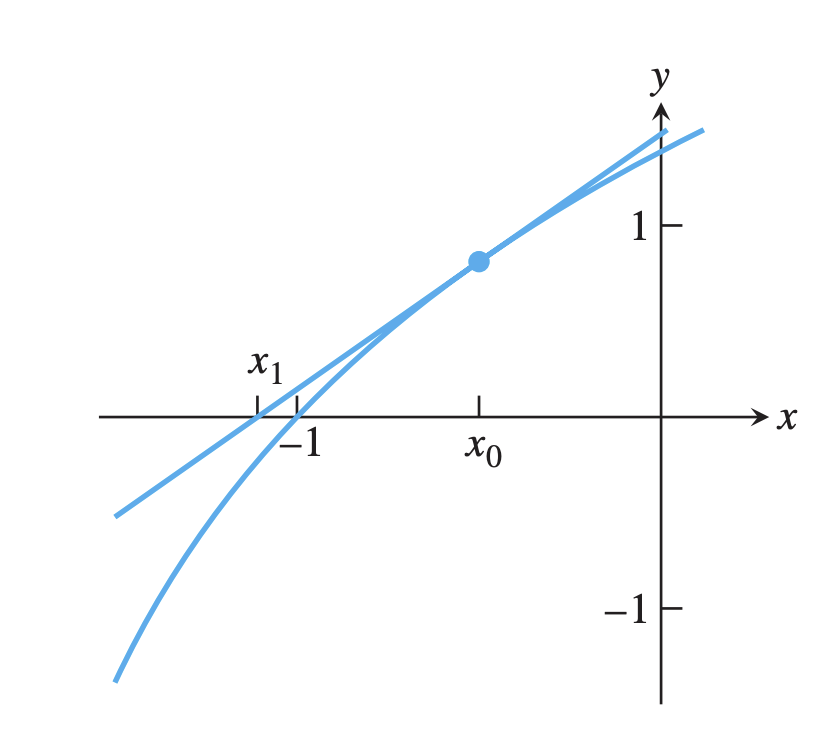
\includegraphics[width=0.25 \textwidth]{img/figure_1_8}
    \caption{One step of Newton’s Method. Starting with x0, the tangent line to the
curve y = f(x) is drawn. The intersection point with the x-axis is x1, the next approximation to the root.}
    \label{fig:1.8}
\end{figure}

From the geometric picture, we can develop an algebraic formula for
Newton’s Method. The tangent line at $x_0$ has slope given by the
derivative $f(x_0)$. One point on the tangent line is $(x_0, f(x_0))$.
The point-slope formula for the equation of a line is:
\begin{equation}
    y - f(x_0) = f'(x_0)(x - x_0)
\end{equation}
so that looking for the intersection point of the tangent line with
the x-axis is the same as substituting $y = 0$ in the line:
\begin{equation}
    f'(x_0)(x - x_0) = 0 - f(x_0)
\end{equation}
\begin{equation}
    x - x_0 = -\frac{f(x_0)}{f'(x_0)}
\end{equation}
\begin{equation}
    x = x_0 - \frac{f(x_0)}{f'(x_0)}
\end{equation}

Solving for $x$ gives an approximation for the root, which we call $x_1$. Next, the entire process is repeated, beginning with $x_1$, to produce $x_2$, and so on, yielding the following iterative formula:

\begin{equation}
    x_0 = \text{initial guess}
\end{equation}
\begin{equation}
    x_{i+1} = x_i - \frac{f(x_i)}{f'(x_i)} \quad \text{for} \quad i = 0, 1, 2, \dots
\end{equation}

\subsubsection{Application of the Newton–Raphson}

In this section we will apply Newton–Raphson in order to solve non-linear equation from our initial problem.

As an initial guesses we will use $p_0 = 0$ and $p_1 = \pi/4$

\vspace{5pt}
\noindent \textbf{Results obtained from the code}
\begin{itemize}
    \item Approximated initial angle:
    \begin{itemize}
        \item $p_0 = 0 \text{ approximation}$: $\theta \approx 0.6567089205736348$
        \item $p_1 = \pi/4 \text{ approximation}$: $\theta \approx 0.6567089205736348$
    \end{itemize}
    \item Number of iterations:
    \begin{itemize}
        \item $p_0 = 0 \text{ iterations}$: $n = 7$
        \item $p_1 = \pi/4 \text{ iterations}$: $n = 8$
    \end{itemize}
    \item Error comparing to the result obtained in Bisection Method part: 
    \begin{itemize}
        \item $p_0 = 0 \text{ error}$: 1.110223024625157e-16
        \item $p_1 = \pi/4 \text{ error}$: 1.110223024625157e-16
    \end{itemize}
\end{itemize}

\vspace{5pt}
\noindent \textbf{Calculation of the order of convergence}

To measure how fast a numerical method finds the exact root, we calculate the order of convergence, $\alpha$. Here is the step-by-step derivation used to find the formula for $\alpha$.

\vspace{5pt}
\noindent \textbf{Step 1: Define the error relationship}

The order of convergence links the error at the next step ($e_{n+1}$) to the error at the current step ($e_n$). This relationship uses an unknown constant number, $C$. The starting formula is:
\begin{equation*}
    |e_{n+1}| \approx C |e_n|^\alpha
\end{equation*}

\vspace{5pt}
\noindent \textbf{Step 2: Use logarithms to separate variables}

We want to find $\alpha$, but we do not know the value of $C$. To fix this, we take the natural logarithm ($\ln$) of both sides of the equation. This gives our first main equation:
\begin{equation*}
    \ln(|e_{n+1}|) \approx \ln(C) + \alpha \ln(|e_n|)
\end{equation*}

\vspace{5pt}
\noindent \textbf{Step 3: Write the equation for the previous step}

This mathematical rule also works for the step right before it. We write a second equation using the error from the previous step ($e_{n-1}$):
\begin{equation*}
    \ln(|e_n|) \approx \ln(C) + \alpha \ln(|e_{n-1}|)
\end{equation*}

\vspace{5pt}
\noindent \textbf{Step 4: Subtract to remove the constant}

We subtract the second equation from the first equation. Because both equations share the term $\ln(C)$, this unknown constant is removed completely from the math:
\begin{equation*}
    \ln(|e_{n+1}|) - \ln(|e_n|) \approx \alpha \big( \ln(|e_n|) - \ln(|e_{n-1}|) \big)
\end{equation*}

\vspace{5pt}
\noindent \textbf{Step 5: Find the final formula} \\
Finally, we use standard logarithm rules to group the terms. We isolate $\alpha$ by dividing both sides. This gives the exact formula to calculate the order of convergence using our lab data:
\begin{equation}
    \alpha \approx \frac{\ln(|e_{n+1}|/|e_n|)}{\ln(|e_n|/|e_{n-1}|)}
\end{equation}

For Newton-Raphson method, for both $p_0$ and $p_1$ initial guesses the order of convergence is quadratic. We can also observe that based on the estimation on every step:

For $p_0$:
\begin{itemize}
    \item step 3: Estimated Alpha = 1.4262
    \item step 4: Estimated Alpha = 1.6712
    \item step 5: Estimated Alpha = 1.9645
    \item step 6: Estimated Alpha = 1.999
    \item step 7: Estimated Alpha = 1.1319
\end{itemize}

For $p_1$:
\begin{itemize}
    \item step 3 Estimated Alpha = 2.3559
    \item step 4 Estimated Alpha = 1.4325
    \item step 5 Estimated Alpha = 1.6651
    \item step 6 Estimated Alpha = 1.9633
    \item step 7 Estimated Alpha = 1.9989
    \item step 8 Estimated Alpha = 1.1573
\end{itemize}

On the last step the value of Alpha significantly decreasing because
of the limited machine precision. The errors are sufficiently small
that machine evaluating their ratio as almost the same.


\subsubsection{Theory of the Secant Method} \cite{Sauer2014}

The Secant Method is a popular technique to find the root of an equation. It is very similar to Newton's Method, but it is easier to use because it does not require calculating the exact derivative of the function.

\vspace{5pt}
\noindent \textbf{How it Works:}

Newton's Method uses a tangent line at one point to find the next guess. The Secant Method replaces this with a ``secant line.'' A secant line is a straight line drawn through the two most recent guess points on the function's graph. The point where this line crosses the zero level becomes the new guess.

\vspace{5pt}
\noindent \textbf{The Formula:}

To calculate the next approximation ($x_{i+1}$), the method uses the difference between the last two points instead of a derivative:
\begin{equation}
    x_{i+1} = x_i - \frac{f(x_i)(x_i - x_{i-1})}{f(x_i) - f(x_{i-1})}
\end{equation}

\begin{figure}[h]
    \centering
    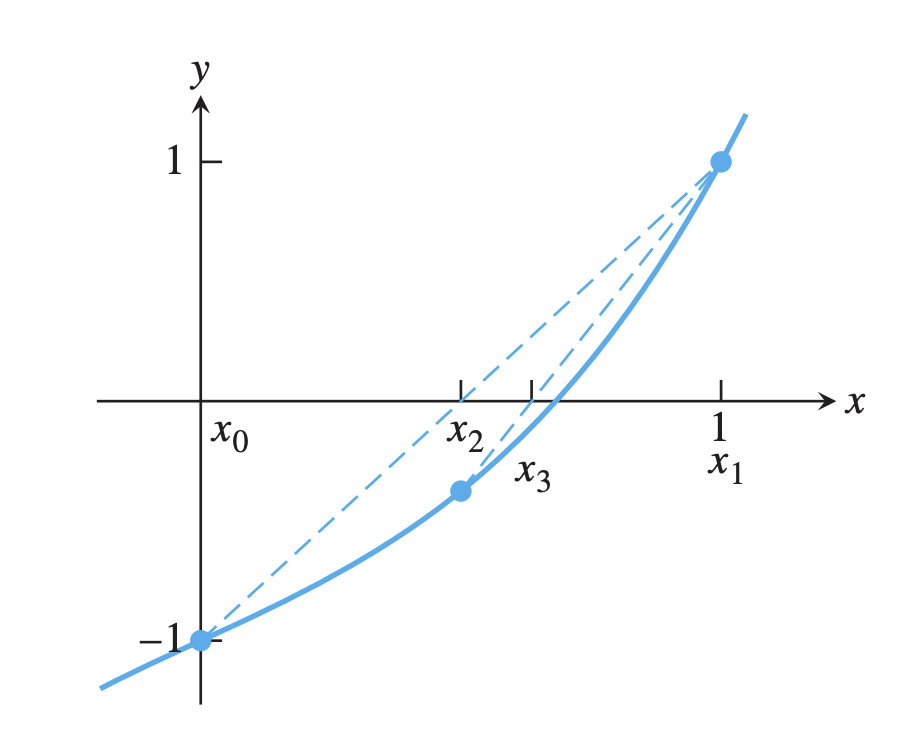
\includegraphics[width=0.25 \textwidth]{img/figure_1_11.png}
    \caption{Two steps of the Secant Method. Illustration of Example 1.16. Starting with $x_0 = 0$ and $x_1 = 1$, the Secant Method iterates are plotted along with the secant lines.}
    \label{fig:1.11}
\end{figure}

\subsubsection{Application of the Secant}

In this section we will apply Secant in order to solve non-linear equation from our initial problem.

As an initial guesses we will use $p_0 = 0$ and $p_1 = \pi/4$

\vspace{5pt}
\noindent \textbf{Results obtained from the code}
\begin{itemize}
    \item Approximated initial angle: $\theta \approx 0.6567089205736352$
    \item Number of iterations: $n = 10$
\end{itemize}

\vspace{5pt}
\noindent \textbf{Calculation of the order of convergence}

To calculate the order of convergence we used the same logic and formulas that were described in the previous section.

For Secant method, the order of convergence was "super" linear ($\alpha \approx 1.6125$). We can also observe that based on the estimation on every step:

\begin{itemize}
    \item step 3 Estimated Alpha = -0.23153
    \item step 4 Estimated Alpha = 6.131
    \item step 5 Estimated Alpha = 0.58335
    \item step 6 Estimated Alpha = 2.3024
    \item step 7 Estimated Alpha = 1.5636
    \item step 8 Estimated Alpha = 1.6302
    \item step 9 Estimated Alpha = 1.6125
    \item step 10 Estimated Alpha = Inf
\end{itemize}

On the last step the value of Alpha significantly decreasing because
of the limited machine precision.







\begin{figure}[h]
    \centering
    
\includegraphics[width=0.25 \textwidth]{bank}
    \caption{Please write your figure caption here.}
    \label{fig:1}
\end{figure}



\subsection{Conclusions}

Here you should discuss obtained results and give corresponding conclusions.

\newpage

\section{Numerical Differentiation \& Numerical Integration}

Describe here the problem which is being investigated in this part. If you want you can copy the text from the lab assignment.  

\subsection{Solution \& Results}

In this section give a theoretical background, describe how you solved the given problem and present your results.

\subsection{Conclusions}

Here you should discuss obtained results and give corresponding conclusions.

\newpage


\section{Interpolation \& Curve Fitting}

Describe here the problem which is being investigated in this part. If you want you can copy the text from the lab assignment.  

\subsection{Solution \& Results}

In this section give a theoretical background, describe how you solved the given problem and present your results.

\subsection{Conclusions}

Here you should discuss obtained results and give corresponding conclusions.


\newpage


\section{Numerical Solution of Differential Equations}

Describe here the problem which is being investigated in this part. If you want you can copy the text from the lab assignment.  

\subsection{Solution \& Results}

In this section give a theoretical background, describe how you solved the given problem and present your results.

\subsection{Conclusions}

Here you should discuss obtained results and give corresponding conclusions.

\newpage

\section*{Declaration of AI Use}

All uses (if any) of AI tools must be declared here. The declaration must include:
\begin{itemize}
\item A statement that AI tools were used and what they were used for (e.g., learning purposes, grammar editing, brainstorming, structuring).
\item A confirmation that the students retain full responsibility for all content.
\item A clear statement that AI was not used to generate solutions of problems, MATLAB codes, analysis and  discussion of results.
\end{itemize}

\newpage

\section*{References}

List all references which you have used. 

\newpage

\section*{Appendix} 

You have to include all your MATLAB functions and scripts here. 
Do not include MATLAB codes as images from a print screen or similar.  Enter your code using the syntax shown below. 

\subsection*{MATLAB codes for Solving Nonlinear Algebraic Equation}

\begin{lstlisting}
% Matlab script for solving nonlinear algebraic equation
close all; clear all; clc;
f=@(x) x.^x;
\end{lstlisting}

\bigskip 

\subsection*{MATLAB codes for Numerical Differentiation \& Numerical Integration}

\begin{lstlisting}
% Matlab script for numerical integration
close all; clear all; clc;
f=@(x) x.^x;
\end{lstlisting}

\bigskip 

\subsection*{MATLAB codes for Interpolation \& Curve Fitting}

\begin{lstlisting}
% Matlab script for curve fitting
x=linspace(0,1,100);
y=x.^3-7*x.^2+14*x-6;
plot(x,y)
\end{lstlisting}

\bigskip

\subsection*{MATLAB codes for Numerical Solution of Differential Equations}

\begin{lstlisting}
% Matlab script for numerical solution of differential equation
close all; clear all; clc;
f=@(x) x.^x;
\end{lstlisting}


\end{document}